\documentclass{bioinfo}
\copyrightyear{2017}
\pubyear{2017}
\usepackage{multicol}

\begin{document}
\firstpage{1}

\title[smt]{\textit{smt}: A High-Performance Software Pipeline for Single-Molecule Tracking}
\author[Yoo \textit{et~al}]{Sun Jay Yoo\,$^{1,2,*}$, Sheng Liu\,$^{3,4,\diamond}$ and Carl Wu\,$^{3,4,\diamond}$}
\address{$^{1}$Department of Biomedical Engineering, Johns Hopkins University\\
$^{2}$Department of Computer Science, Johns Hopkins University\\
$^{3}$Department of Molecular Biology \& Genetics, Johns Hopkins University School of Medicine\\
$^{4}$Department of Biology, Johns Hopkins University}

\history{Received on December 20, 2017}

\editor{* Author for correspondence (e-mail: syoo21@jhu.edu) \\ $\diamond$ Faculty corrspondence (e-mail: sliu@jhu.edu, wuc@jhu.edu)}

\maketitle

\begin{abstract}
\textit{smt} is a single-molecule tracking analysis software and graphical user interface built as an R package. In order to allow users to derive cause-and-effect relationships from single-molecule kinetics and build mechanistic cellular models from super-resolution fluorescent microscopy, \textit{smt} aims to provide a full suite of analytic tools that turns tracking data into meaningful statistical results. 

\textit{smt} can first be used to read and process raw particle output from various localization software into a versatile format that can be further refined, saved, and analyzed. \textit{smt} currently supports the Diatrack, MosaicSuite, and SLIMFAST software. Users are then granted tools such as trimming, filtering, linking, merging, and masking to remove noise and selectively choose target data. All track data can be dynamically visualized individually or as time-stacked videos to qualitatively assess macroscopic cellular dynamics. \textit{smt} also supports a multitude of quantitative statistical tools to analyze single-molecule data effectively and accurately. Calculations such as the mean square displacement and the diffusion coeffient are supported along with other tools such as hidden Markov models, cumulative distribution function fits, normal distribution fits, dwell time, and kernel density. \textit{smt} takes full advantage of high-performance, multi-cluster computing units and optimizes intensive operations for parallel computation for maximum efficiency in both the package and the graphical user interface.

As an integrated software, \textit{smt} aims to unify the many steps in the single-molecule tracking pipeline and provide a simple method for statistical analysis.
\end{abstract}
%%%%%%%%%%%%%%%%%%%%%%%%%%%%%%%%%%%%%%%%%%%%%%%%%%%%%%%%%%%%%%%%%%%%%%%%%%%%%%%%%%%%%%%%%%%%%%%%%%%%%%%%%%%%%%%%%%%%%%%%%%%%%%%%%%%%%%%%%%%%%%%%%%%%%%%%%%%%%%%%%%%%%%%%%%%%%%%%%%%%%%%%%%%%%%%%
\section{Introduction}


With the advent of super-resolution single-molecule imaging and the acquisition of high-performance computing power in biophysics laboratories, there is an increased dependence on software pipelines to answer specific questions raised by biomedical researchers on cellular processes. Specifically, the ability of researchers to use fluorescent bio-markers and tags to study real-time, live-cell visualization of individual molecules at high spatiotemporal resolution, avoiding fixation artifacts, has been largely successful in prokaryotic and eukaryotic systems \citep{Liu}. By cross-validating and integrating data from single-molecule experiments from in vivo and ex vivo approaches, there is newfound potential to generate mechanistic and conceptual models to reveal the underlying logic for cell processes, namely chromatin-based regulation of eukaryotic transcription.

\begin{figure}[b]
\centerline{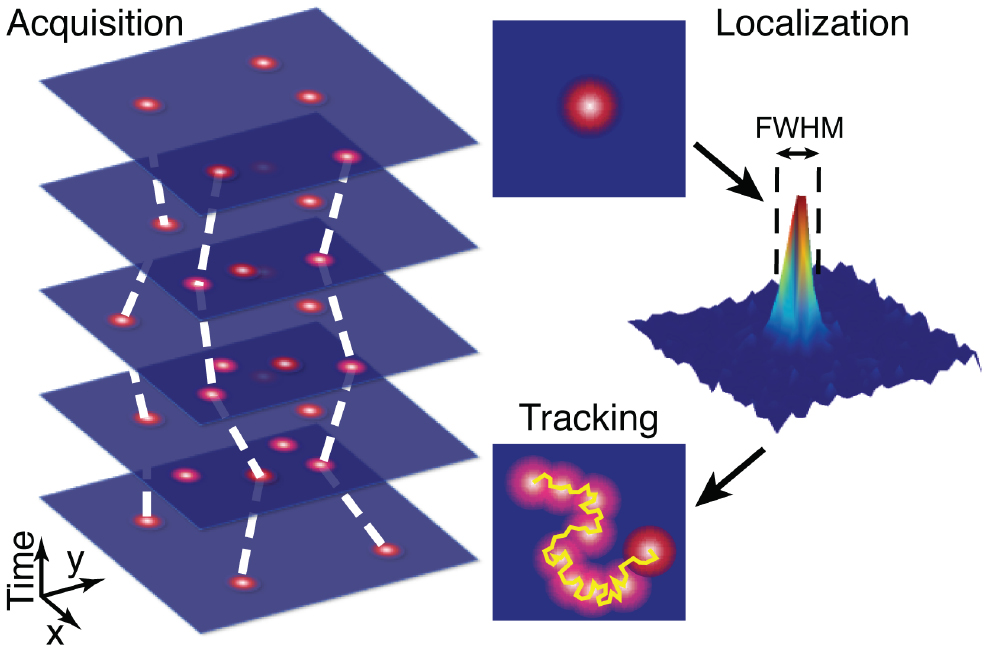
\includegraphics[width=60mm]{local.jpg}}
\caption{Schematic diagram of single-molecule tracking and localization \citep{Manzo}. During acquisition, series of incidence images are taken to form a video. During localization, an ideal point-spread function of a single emitter is compared to the realized experimental intensity to characterize a Gaussian fit localized to a sub-diffraction limited area. These positions across time have the potential to be linked into a track.}\label{fig:01}
\end{figure}

\begin{figure*}[!tpb]
\centerline{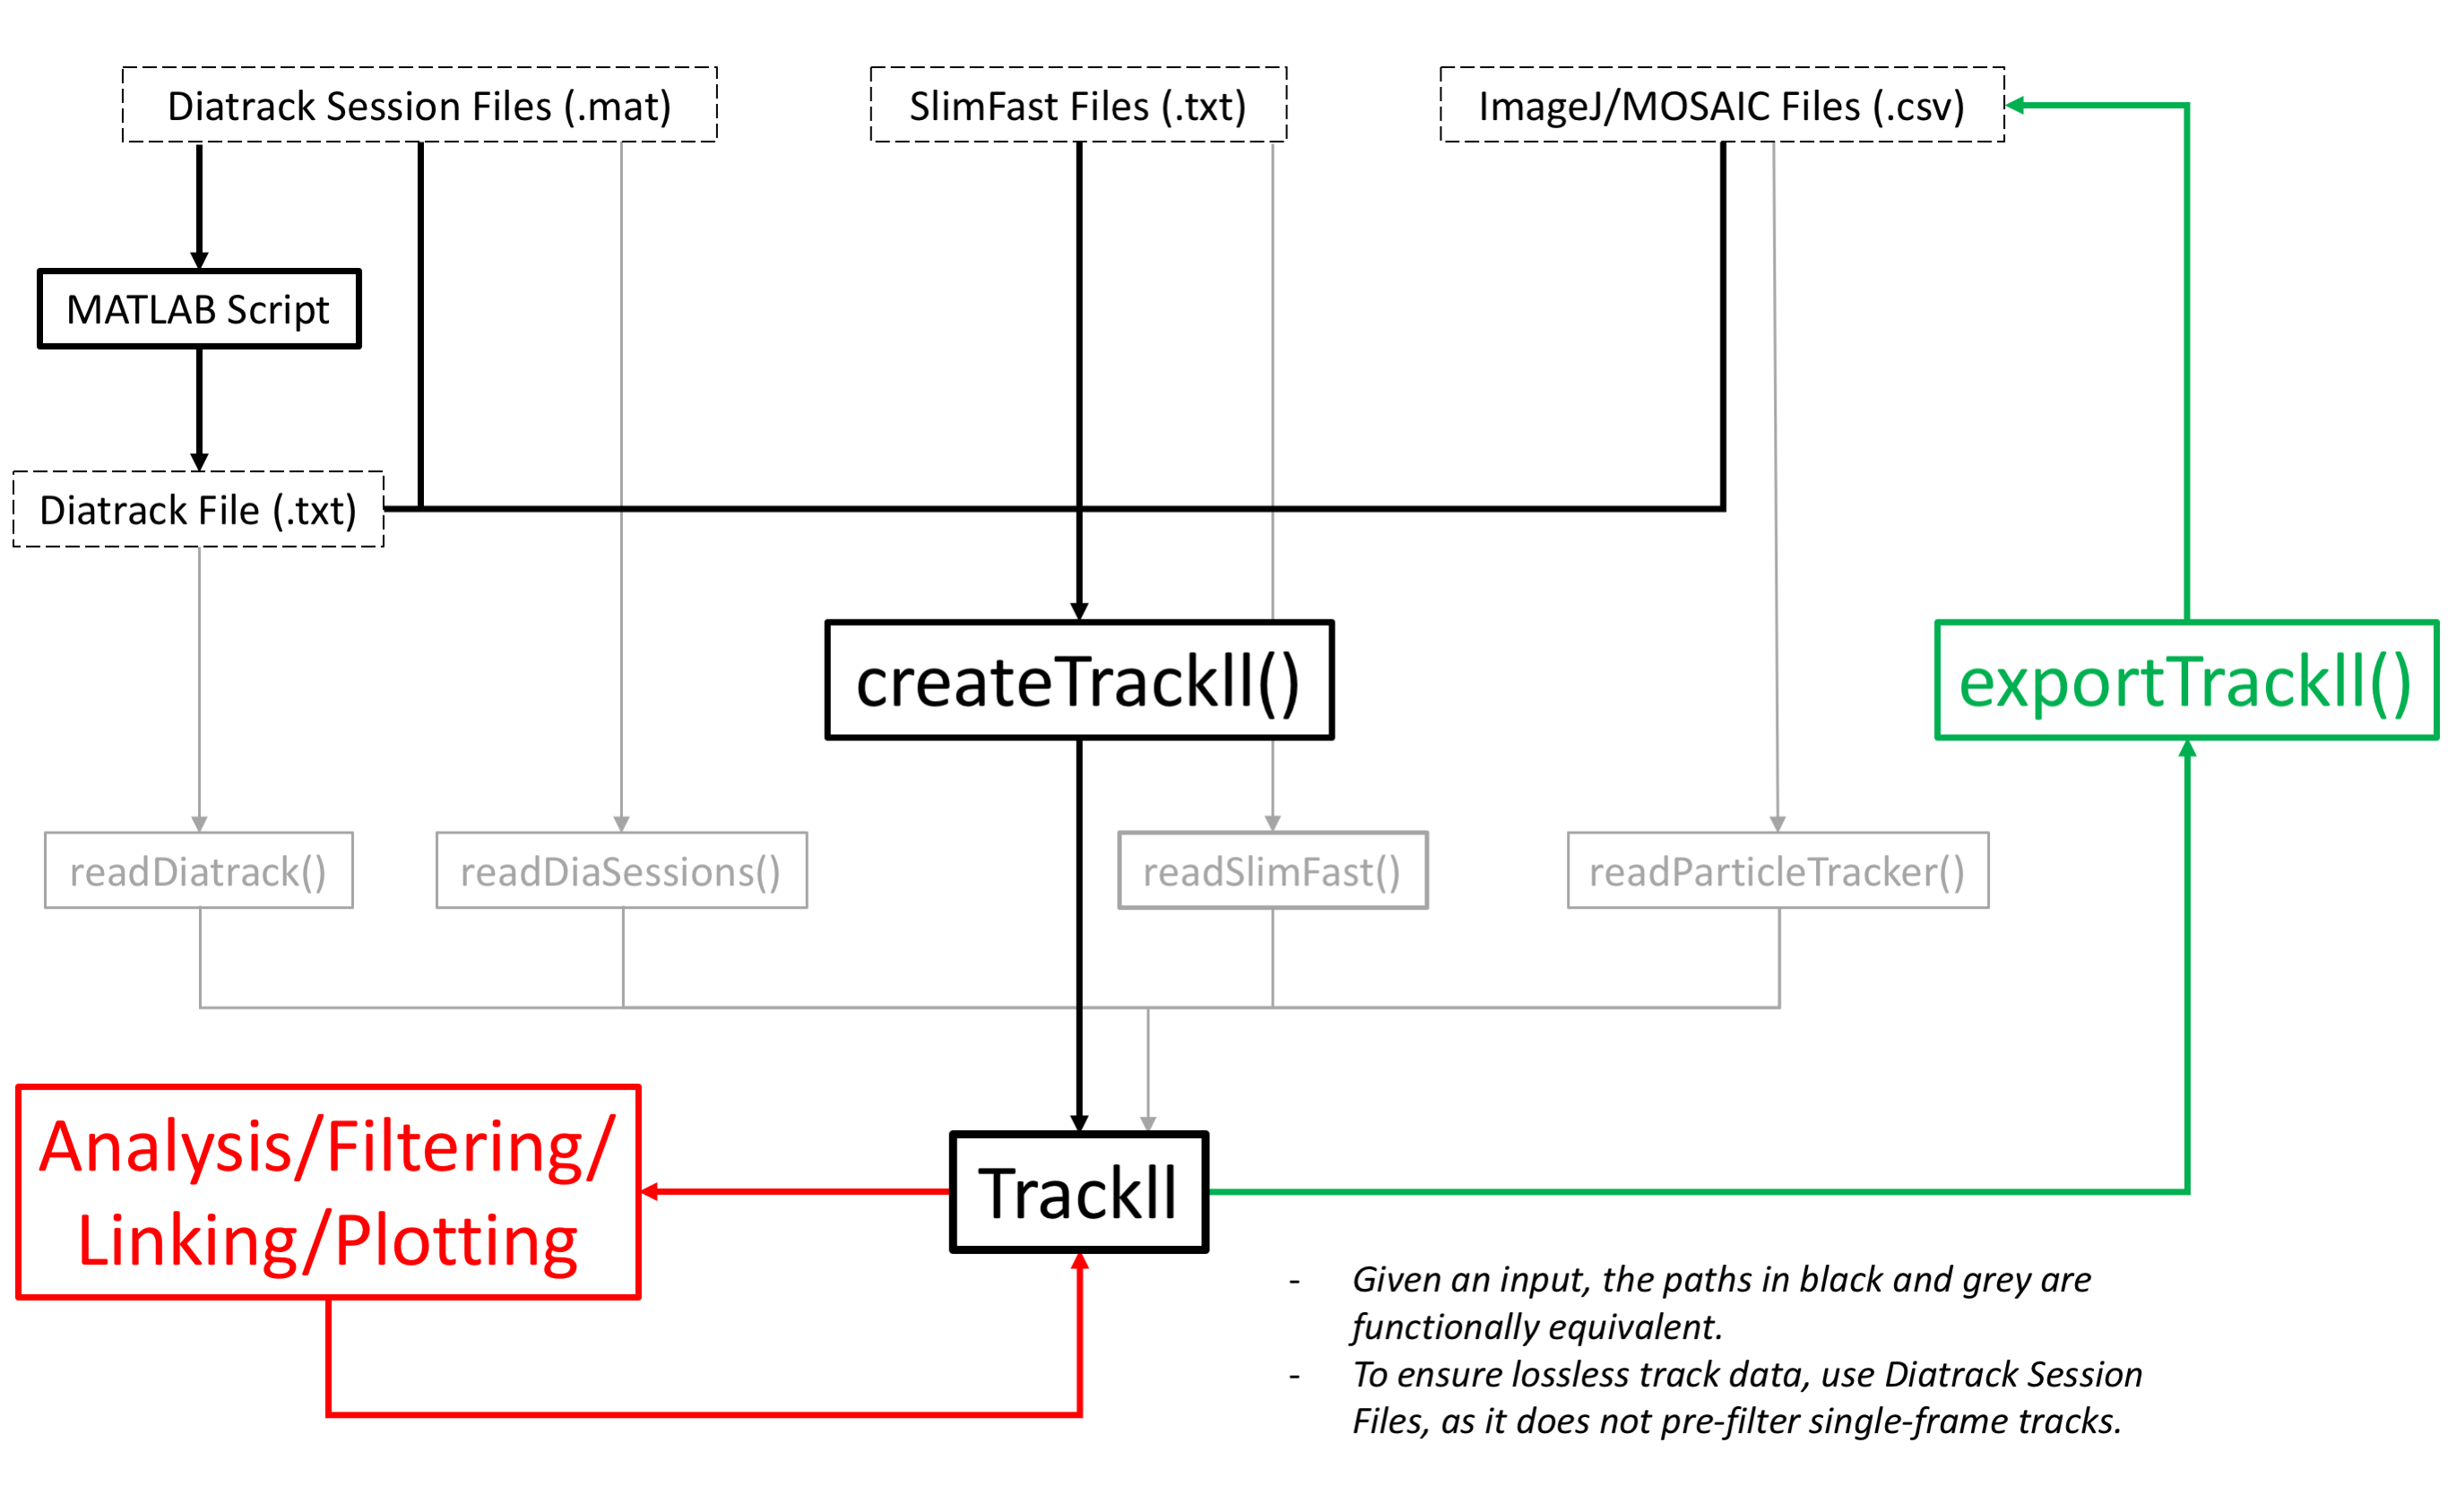
\includegraphics[width=120mm]{pipeline.png}}
\caption{Diagram illustrating the general workflow structure of reading, analyzing and exporting raw track data. Raw data is inputted as a form of Diatrack MATLAB files, SLIM-FAST text files, or MosaicSuite CSVs but nonetheless get processed the same downstream.}\label{fig:02}
\end{figure*}

By using live-cell imaging of custom single fluorescent HaloTag-JF protein fusions (high affinity chemical ligands linked to bright organic fluorophores, developed in the collaborating HHMI-Janelia), we are able to determine the positions of these tags in nanometer ($\sim$30 nm) resolution and track particle movements in two dimensions at millisecond ($\sim$10 ms) temporal resolution. This imaging modality uses stochastic flurophore activation (STORM) at high laser intensity with short (10 ms) camera exposures to capture both slow (chromatin-bound) and fast (chromatin-free) diffusing molecules. Using low laser power and long exposures ($\sim$500 ms), we can exclude fast diffusing particles by motion blur and quantify chromatin-bound molecule lifetime. Lastly, high laser power imaging using time-correlated photo-activated localization microscopy (tcPALM) can reveal highly transient spatial clustering of photo-active fluorescent protein molecules. Thus, the imaging and biological technology available has a huge potential to study the real-time dynamics of cellular processes in nuclear space.

However, there is a severe lack of software needed to support such high-throughput data and researchers are limited in the number of statistical tools at their disposal to make meaningful conclusions. We aim to fill that technological gap by providing a downstream computational pipeline for statistical analysis to take advantage of this super-resolution imaging modality and access to high-performance computing units. In conjunction with existing particle-tracking software such as Diatrack, MosaicSuite, and SLIM-FAST, it is possible to extract particle movement data through two-dimensional Gaussian fits, as shown in Figure \ref{fig:01}. This data, along with raw single-molecule images, was readily available for us in shared servers and the computing power to process such data was easily accessible through custom high-performance compute clusters. Using R, we will be developing a whole suite of statistical and computer vision tools, packaged in a easy-to-use graphical user interface, to provide downstream analysis of imaging data. The result is to hopefully provide a clean and unified method to simplify the process from data acquisition to data analysis and provide useful analytic tools such as mean square displacement, density coefficients, hidden Markov models, and more.

\begin{figure}[b]
\centerline{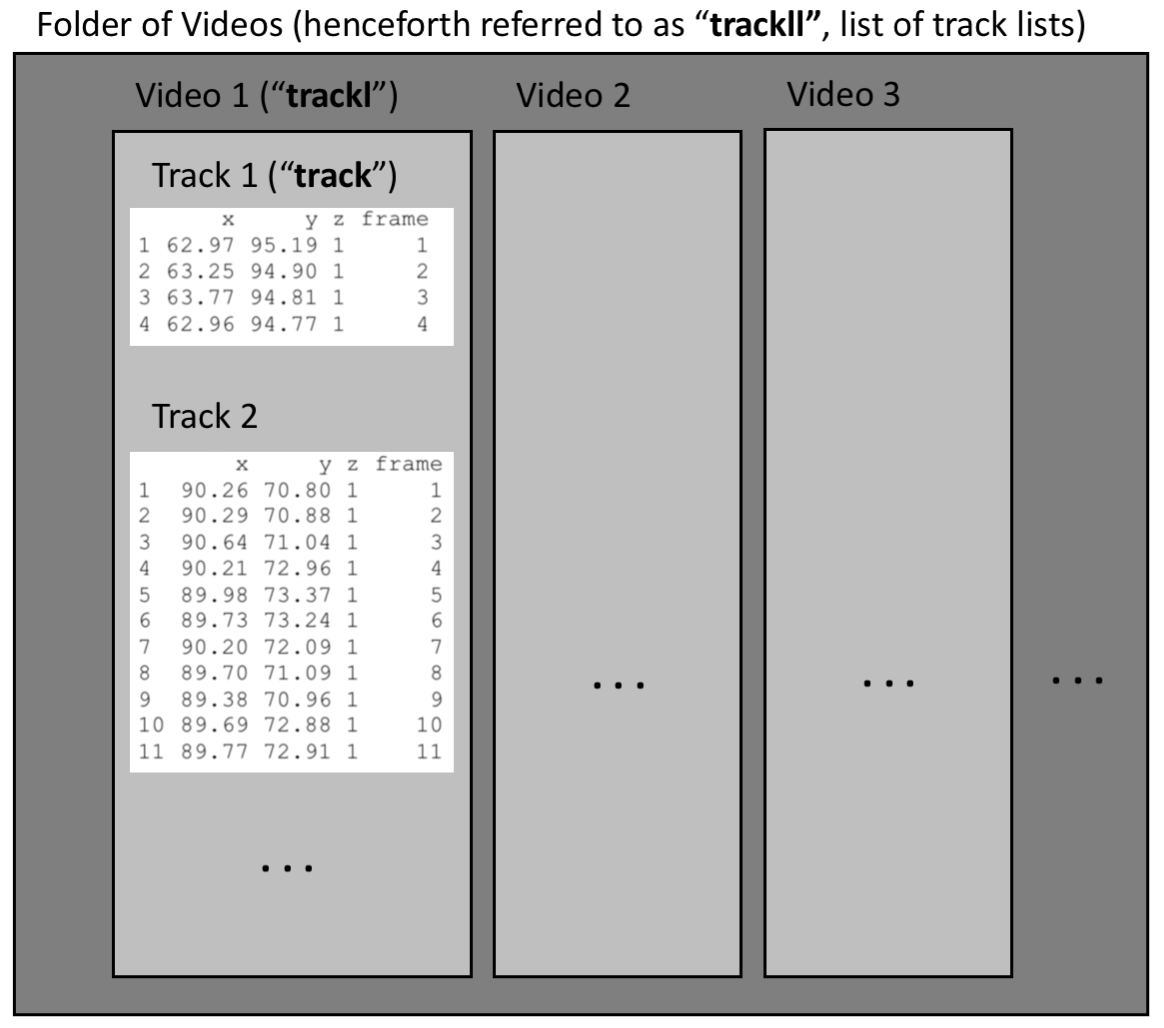
\includegraphics[width=75mm]{ds.png}}
\caption{Illustration of the software's primary data structure hierarchy such that trackll $\ni$ trackl $\ni$ track.}\label{fig:03}
\end{figure}

%%%%%%%%%%%%%%%%%%%%%%%%%%%%%%%%%%%%%%%%%%%%%%%%%%%%%%%%%%%%%%%%%%%%%%%%%%%%%%%%%%%%%%%%%%%%%%%%%%%%%%%%%%%%%%%%%%%%%%%%%%%%%%%%%%%%%%%%%%%%%%%%%%%%%%%%%%%%%%%%%%%%%%%%%%%%%%%%%%%%%%%%%%%%%%%%
%\begin{methods}
\section{Methods}

\subsection{Overview}

\begin{figure*}[t]
\centerline{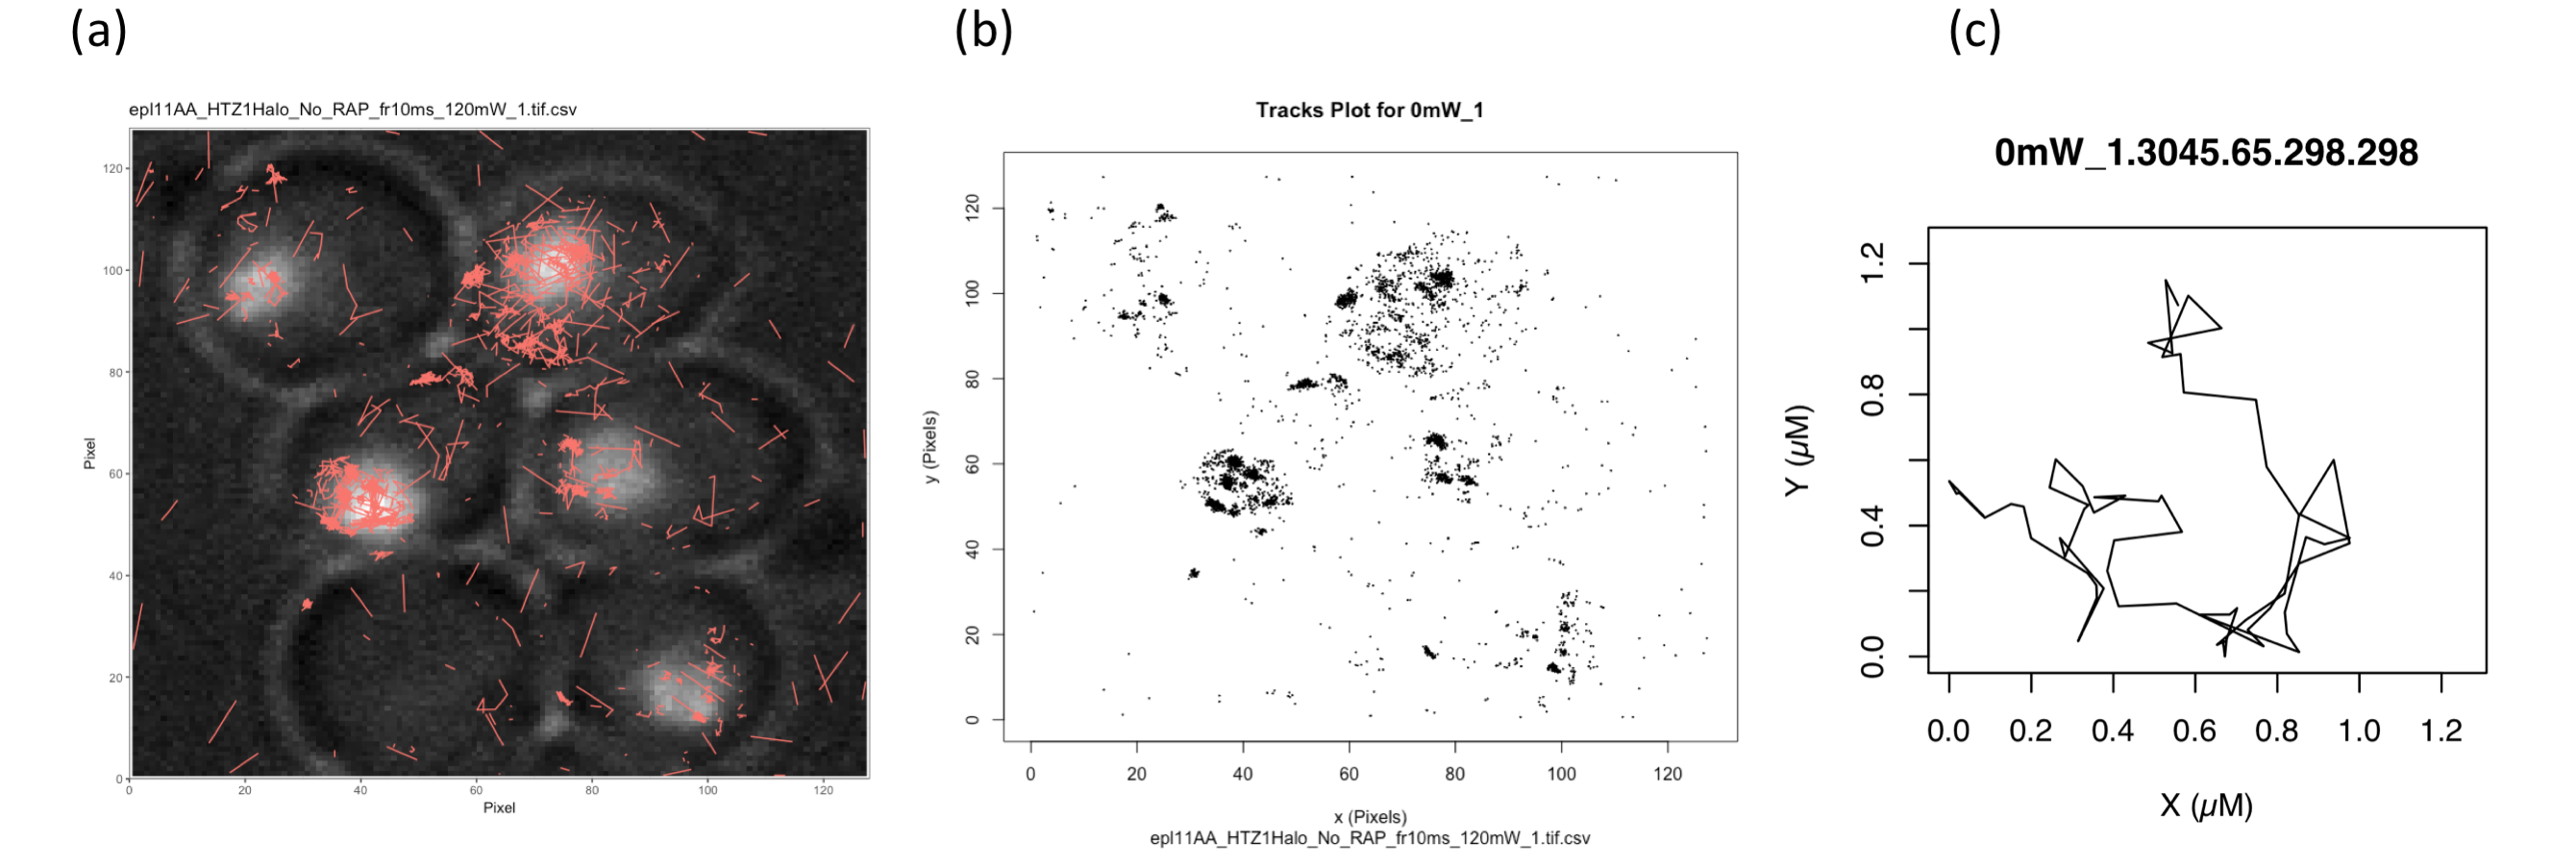
\includegraphics[width=180mm]{plot.png}}
\caption{Plotting methods included in \textit{smt} with sample raw data in a 128x128 pixel region. (a) Plot of complete time-stacked track trajectory lines over a cell overlay taken with a high-intensity flash in the first few seconds of imaging. (b) Plot of all single-molecule incidences in a complete time-stack. (c) Plot of an individual track against an absolute coordinate.}\label{fig:04}
\end{figure*}

\textit{smt} (single-molecule tracking) is a R software package and graphical user interface that aims to take single-molecule tracking data processed from multiple existing single-molecule localization software (eg. Diatrack, MosaicSuite, SLIM-FAST) and transform it into a format that can be easily read, refined, and analyzed. The software allows users to easily upload raw localization data and supports saving and re-reading of processed data for long-term data management. Furthermore, the analysis techniques currently supported by the software allows all graphs and parameters describing single-molecule kinetics to be exported in a presentable and efficient manner. The general software pipeline of the software can be seen in Figure \ref{fig:02}. Computationally heavy tasks makes use of multi-core and multi-cluster machines with parallel programming and memory allocation is minimized to preserve full functionality. The simplicity of the package design allows the package to be used remotely on a R-Studio Server (file server and remote workstation setups) and supports a full graphical user interface for non-coders that can be run either locally or in a Shiny web server. The following sections aim to describe the core features in \textit{smt} spanning across the software pipeline from data acquisition to data analysis.

\subsection{Reading Single-Molecule Tracks}

While the software fully supports processing a single, lone video of a cell population, we found that it was much more common for researchers to image multiple cell populations at once and produce multiple videos for batch analysis. As non-autonomous super-resolution imaging is the time-limiting step in the single-molecule tracking pipeline, it was highly preferred to gather as many imaging videos as possible before proceeding to localization and downstream \textit{smt}. Furthermore, as the set of videos are either for collective sampling or comparative analysis, there was a need for a method to organize this data into a simple data structure hierarchy.

The highest-level in this structure is the ``folder" that contains the videos of the target cells. The next level of this hierarchy is therefore the ``video". As each video contains the information for all the single-molecule trajectories that appear in that session, the next level of the hierarchy is the ``track". Each track is a data frame that keeps record of a single particle trajectory. This data frame contains essential information such as the x-y pixel data and the frame number of appearance, but it also contains miscellaneous information such as emission intensity and Gaussian goodness-of-fit (depending on the localization software used) for future in-depth analysis. Each folder is referred to as ``trackll" (list of track lists), each video as ``trackl, and each trajectory within the video as ``track" (Figure \ref{fig:03}). This data structure described is the unique form that is kept throughout the entire pipeline, as it can be modified, analyzed, and saved for record-keeping and raw-data visualization.

In order to create such a final structure, individual reading algorithms were built to support each type of localization input with the ``read" functions. However, in order to increase usability and support scalability to other localization and tracking data types, a general purpose reading function was created (see \textit{createTrackll()} in Figure \ref{fig:02}). This function automates the data-type selection process and initiates parallel execution to read the given localization data into the described data structure. Because single-molecule localization software is typically highly variable in terms of features, accuracy, usability, method of localization, and pipeline integration, this independence from associated localization software allows for simplicity and automation in the reading process. Furthermore, supporting more localization software and their produced data types typically only require development of a short reading algorithm that can be easily integrated into the general purpose reading algorithm.

\begin{figure*}[!tpb]
\centerline{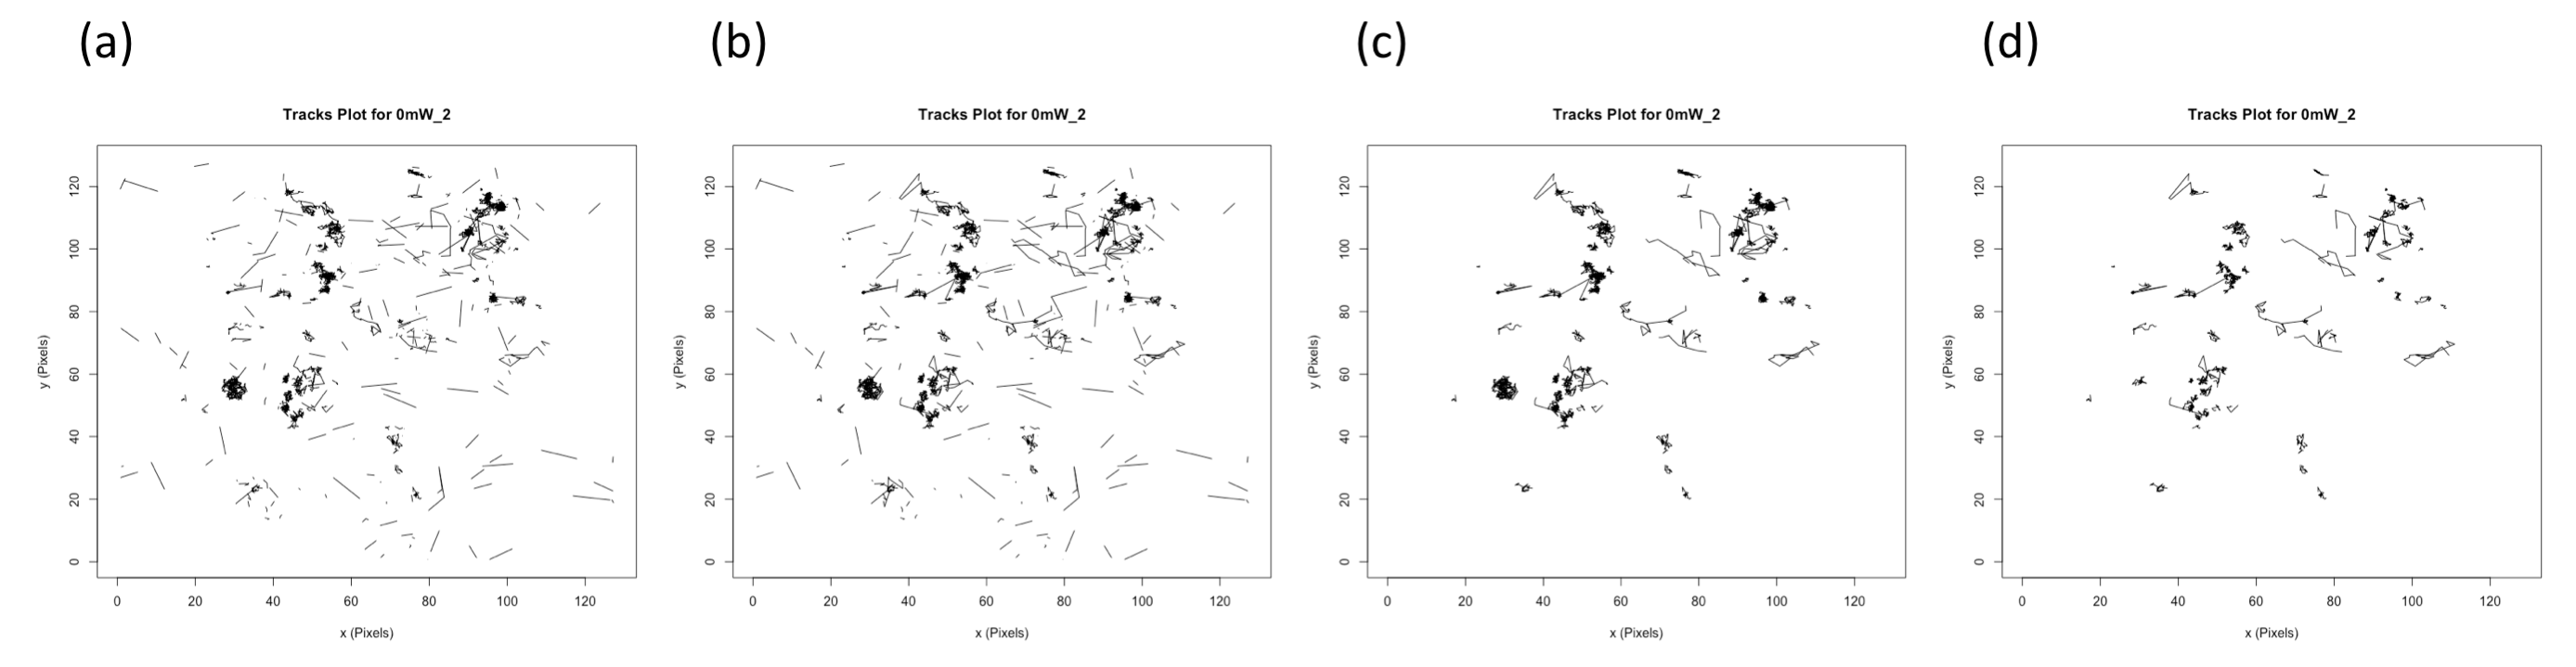
\includegraphics[width=185mm]{refine.png}}
\caption{Preliminary track refinement of sample data using linking, filtering and trimming. (a) Plot of raw data without any refinement. (b) Plot of tracks with linking at a tolerance of 5 pixels and a maximum frame skip value of 10 frames. (c) Plot of tracks with linking and filtering at only those with a length of seven frames to infinity. (d) Plot of tracks with linking, filtering, and trimming to a maximum frame length up to 32 frames.}\label{fig:05}
\end{figure*}

Lastly, in order to best support the graphic visualization of tracks, plotting entire time-stacked videos on a cell overlay, plotting all single-molecule incidences, and plotting single tracks are all fully supported at any point if the software pipeline. Plotting over a cell image overlay is especially useful as a sanity check during reading and processing, but note that static cell images shot during the first few seconds of imaging are not indicative of the cell and nucleus's location throughout the span of the video. Figure \ref{fig:04} depicts raw sample data plotted with these multiple methods before any refinement.

\subsection{Refining Tracks and Censoring Noise}

With the rise of single-molecule tracking, there has been a monumental shift to imaging transcription as it embodies an insightful application of this technology. While traditional genetic, genomic, and biochemical methods have proved successful in studying factors, regulatory sequences, and associated pathways that modulate transcription, they typically only provide snapshots of the population dynamics behind the stochastic biochemical process of transcription regulation. Live single-molecule tracking has thus become a complementary technique to observe molecular events involved in transcription in real-time and derive causal relationships from quantitative kinetics to build predictive models for transcription \citep{Coleman}. As studies of chromatin components and their transactions in transcription regulation deeply focus on kinetics that occur in the nuclei, single-molecule incidences that occur outside the nuclei must be filtered and removed. Furthermore, as certain fluorescent tags and their associated complexes have varying lifetimes, prolonged tracks can also be censored. As both biological and experimental constraints compel favoring of certain tracks over others, methods to refine tracks and censor noise, while preserving the primary data structure, were developed downstream to the initial reading of raw incidences. Figure \ref{fig:05} depicts a several of the steps of track refinement and the rest of this subsection is dedicated to describing these various methods of processing.


\subsubsection{Filtering and Trimming}

Filtering and trimming is as the name implies. As track data records the incident frames, the time in frame length can be calculated for each track. Filtering merely eliminates all tracks that does not pass through a desired filtered length range. In order to selectively keep tracks existing for longer times, users can select a range from length \textit{x} to infinity. All tracks less than the length \textit{x} will be eliminated. Trimming takes every track and trims it to a desired length. This is especially useful if the tag is known to have a certain decay period or if a uniform track length is needed for downstream unbiased statistical analysis.


\subsubsection{Linking}

As high laser intensity STORM imaging can typically only record in $\sim$10 ms exposures per frame, localization software packages are often limited in their ability to precisely link tracks. Not only are tracks that disappear and reappear after a few frames always regarded as two separate particle tracks, but the track linking sensitivity needs to often be adjusted beyond the Gaussian fit. Thus, a linking method was created to best account for these limitations. Linking skipped frames takes in parameters such as absolute tolerance distance and maximum skipped frames to link tracks that should theoretically be considered as one single-molecule trajectory. These parameters vary according to the particular fluorophores and the imaging technique, but \citealp{Plank}, for example, theorized that CyPet had a localization precision of $\sim$50 nm across a theoretical limit of 10 skipped frames for reappearance.

\begin{figure}[!tpb]
\centerline{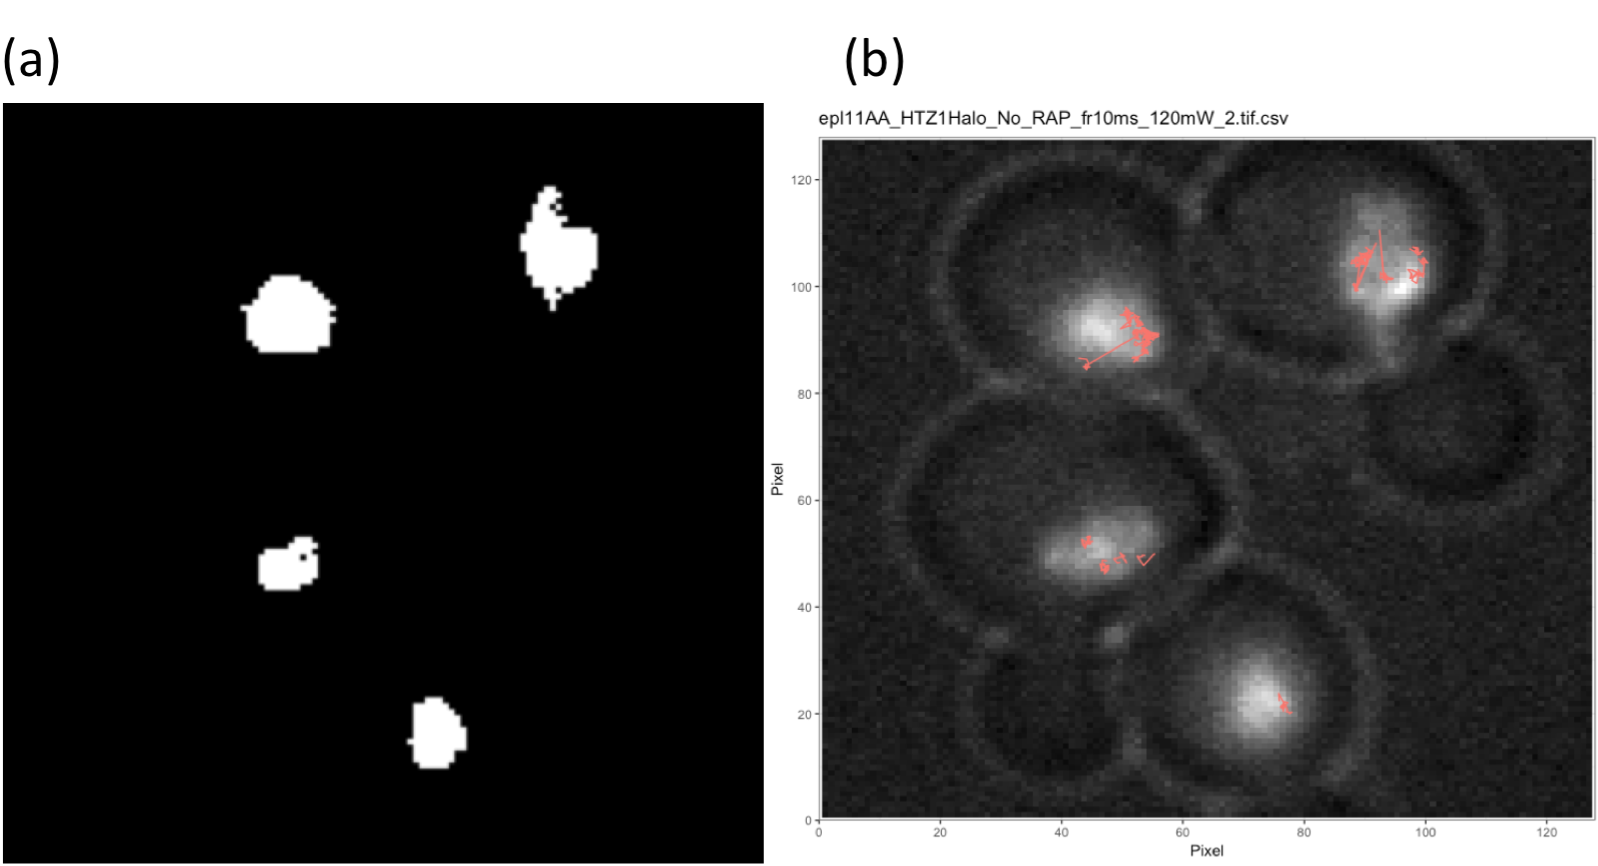
\includegraphics[width=75mm]{mask1.png}}
\caption{Binary threshold masking using data from Figure \ref{fig:05}(d). (a) Binary image mask manually created through 8-bit thresholds in FIJI (b) Resulting track plot with extranuclear tracks censored and masked. (c) Overlay of resulting masked tracks on the original nuclear overlay for verification.}\label{fig:06}
\end{figure}

\begin{figure}[!tpb]
\centerline{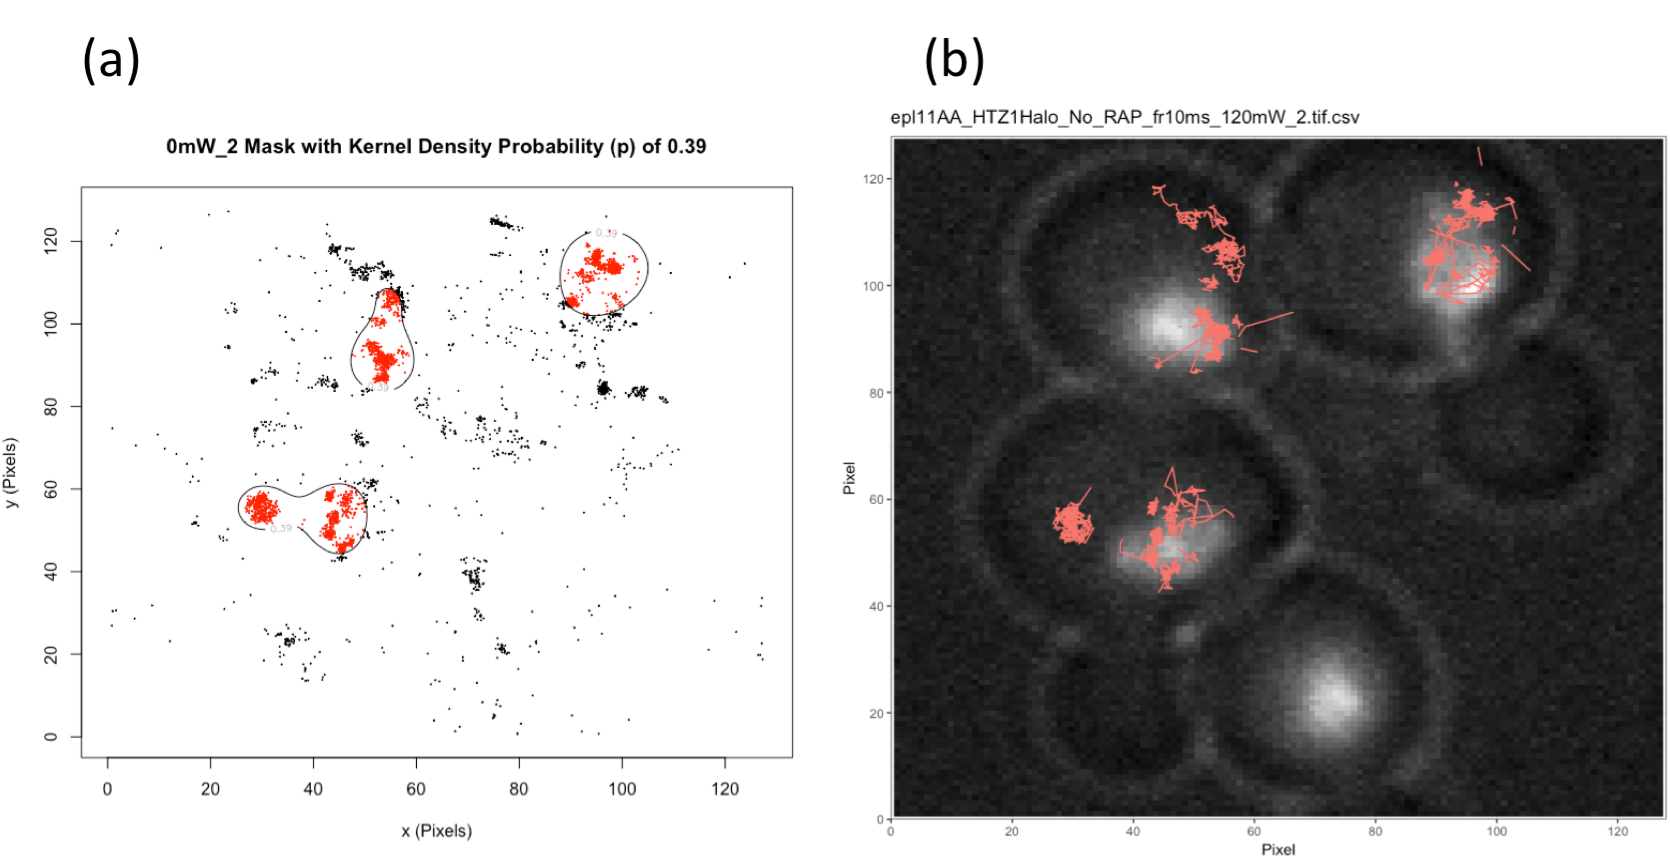
\includegraphics[width=80mm]{mask2.png}}
\caption{Kernel density masking using data from Figure \ref{fig:05}(d). (a) Single-molecule incidences with density contour plot in red. (b) Resulting track plot after density masking. (c) Overlay of resulting masked tracks on the original nuclear overlay for verification.}\label{fig:07}
\end{figure}

\subsubsection{Merging}

Merging is a purely organizational tool that collates all the tracks in the ``trackll" data structure (the list of track lists) into a single track list. This is to support combining multiple videos from the same cell sample into one grouping for increased accuracy and reliability of downstream analysis tools. These ``trackl" (merged track list) can then be combined with other track lists to reform the original ``trackll" data structure.

\subsubsection{Masking}

While the previously described methods of track processing (Figure \ref{fig:05}) are rather independent of cell nuclei and the track's spatial distribution, masking aims to censor ``noise" tracks by best estimating the location of the nuclei or the target site within the optical field of view. The following describes the two methods of masking integrated into \textit{smt} shown in Figure \ref{fig:06} and Figure \ref{fig:07}.

The first method of segmentation supported by \textit{smt} is manual masking through image thresholds. Given the STORM microscopy regiment, it is possible to take advantage of the high-intensity laser flash to capture a rough visual of the cell specimens before beginning any single-molecule tracking. This initial glow gives an approximate visualization of the cell and its nuclei at that particular time. Taking this image and applying 8-bit intensity threshold in image processing software such as FIJI/ImageJ allows one to manually create a binary image mask of the nuclear glow that can be used to censor tracks appearing outside the predefined area (Figure \ref{fig:06}). It is important to note that this method does not account for nuclear movement throughout the imaging session and poses large inaccuracies for edge tracks upon imprecise thresholds.

The second method of segmentation is the process of masking through the spatial density of single-molecule incidences for the full time-stack. This method aims to alleviate the limitations of manual binary masking, as it does not rely on any nuclear image and solely depends on track data. The assumption (and therefore, limitation) of this method is that dense regions of single-molecule incidences are relatively good predictors of nuclear regions-of-interests. As lice-cell nuclei often shift during imaging, filtering out tracks located only in denser regions in the field of view is theorized to be an improved method to mask out noise. While two-dimensional binning was first considered to be a simple way to assess densities, it was quickly noted that density estimations became wildly irregular and variable depending on the reference frame and the natural variance from different imaging modalities. The method-of-choice was to remove the histogram binning completely and instead sum kernels that are centered at each single-molecule incidence. This summation of these kernels result in a kernel density estimate (KDE) for the spatial density of the single-molecule tracks. While this method allowed for accurate density monitoring, it still required a kernel density probability to actively select desired regions in track data of varying sparsities.

The specific method chosen was a generalization of the multivariate KDE to bivariate, 2-D data \citep{Venables}. For a bivariate random sample $X_1, X_2, X_3,..., X_n$ selected from a density $f$, the KDE can be modeled to be:

\begin{equation}
\hat{f}_H(x) = \frac{1}{n}\sum_{i=1}^{n}K_H(x-X_i)
\end{equation}

where $x = (x_1, x_2)^T$ represents transposed bivariate pixel data, $X_i = (X_{i1}, X_{i2})^T$, and $i = 1, 2,...,n$. In this case $K(x)$ is the kernel window function of the symmetric probability density function and $H$ plays the role of the covariance matrix as a bandwidth matrix which is both symmetric and positive-definite. The choice of $K$ was not crucial in this case and was chosen to be the standard two-dimensional normal:

\begin{equation}
K(x) = \frac{1}{2 \pi} \exp(-\frac{1}{2}x^Tx) 
\end{equation}

The choice of $H$ was crucial in determining the performance of $\hat{f}$, thus the unconstrained common parameterization of the diagonalized variance matrix was used, such that:

\begin{equation}
H =
\quad
\begin{bmatrix} 
h_1^2 & 0 \\
0 & h_2^2 
\end{bmatrix}
\end{equation}

Using this bivariate KDE, a binary mask was then created using only complete contour polygons. While this method was robust in masking for known kernel density probabilities, many test cases involved variations in the probability ranging from around 0.2 to 0.9. Thus, a unified system was built into \textit{smt} in order to build a regression model to predict for kernel density probabilities given a set of video samples originating from the same cell population. From empirical data from varying cell types, imaging modalities, and localization software, it was clear that average track lengths of raw data was an incredible linear predictor of kernel density probabilities with $R^2 > 0.98$ in almost all cases. Even though full automated probability estimation is difficult with previously unused flurophore tags, imaging techniques, and etc., it was theorized that the unique regression model created for each cell type and imaging technique can be generalized to all videos in that population. \textit{smt} allows users to dynamically build a model that gradually improves with each manual probability adjustment. In a set of 40 videos, for instance, after manually tuning even the first 10 videos, the remaining 30 could be masked automatically and accurately using this unique regression model. This model can be saved, adjusted, and reused/rebuilt for future samples. Figure \ref{fig:08} shows examples of what automated kernel density probability estimations and masking might look like for new videos shot from the same cell sample with a regression model containing 10 previously adjusted probability estimations and their average track lengths. While not all imaging techniques produce data of this quality, Figures \ref{fig:08}(a), \ref{fig:08}(b), and \ref{fig:08}(d) visually show clear nuclear and cell membranes from single-molecule incidences. Figure \ref{fig:08}(c) shows typical density variations even within the same cell sample and how a reduction of intrinsic noise can lead to wildly higher probability estimates.

\begin{figure}[!tpb]
\centerline{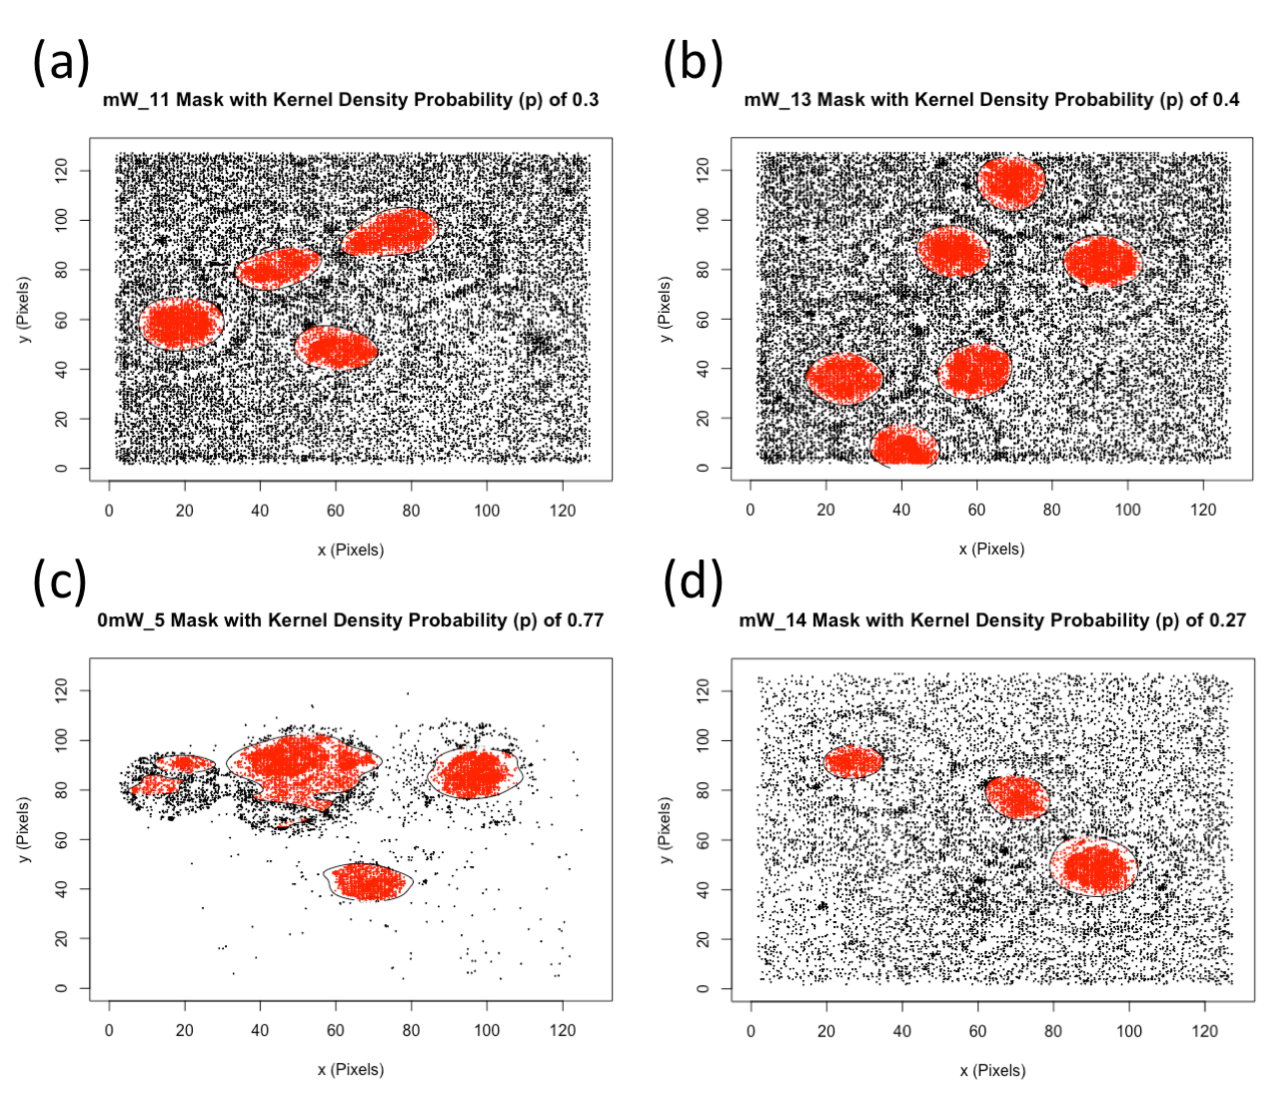
\includegraphics[width=90mm]{kd.png}}
\caption{Automated kernel density masking of four videos with cells from the same sample population. In order automate density masking, a regression model was interactively built from ten previously seen track plots. (a) Masking with a probability of 0.3. (b) Masking with a probability of 0.4. (c) Masking with a probability of 0.77. (d) Masking with a probability of 0.27.}\label{fig:08}
\end{figure}


\subsection{Analyzing Tracks}

After tracks have been read and refined, they can be analyzed through various statistical methods. While there are an unbounded number of ways to analyze such data, there are five main methods of analysis that were found to be most useful for studying cellular mechanics and kinetics. Methods such as the mean square displacement, diffusion coefficient, and dwell time study the tracks on the trajectory level, methods such as the CDF fit study the tracks on a single-step basis, and methods such as hidden Markov models study tracks through track states.

\subsubsection{Mean Square Displacement}


The mean square displacement (MSD) is a measurement for the average displacements of a particle tracked over an incremental time interval. In statistical mechanics, the MSD can be thought of as a common measure for the spatial coverage of Brownian motion -- the amount of system explored by a mathematical ``random walk". From the MSD, the behavior and type of diffusive motion that the particle follows can be ascertained by plotting it against the number of time intervals analyzed. The formal definition of the MSD relies on the notion that a single particle track is a sequence of $N$ positions $\big\{r_i\big\}^N_{i=1} = \big\{x_i, y_i\big\}^N_{i=1}$ observed at times $\big\{t_i\big\}^N_{i=1}$ separated by time steps $dt$. The MSD is then calculated for time intervals $\tau$ as such \citep{Vrljic}:

\begin{align}
    MSD(\tau) & \equiv \Big \langle \Delta r^2(\tau) \Big \rangle \label{eq:04} \\ 
    & =  \Big \langle |r_{i+\tau} - r_i|^2 \Big \rangle \label{eq:05} \\ 
    & = \frac{\sum_{i=1}^{N-\tau}\big \langle (x_{i+\tau} - x_i)^2  + (y_{i+\tau} - y_i)^2 \big \rangle}{N - \tau} \label{eq:06}
\end{align}

The MSD is the vector distance ($r$) traveled by a particle over some time intervals ($\tau$) (Equation \ref{eq:04}). The square displacement from position $i$ to $i+\tau$ is averaged over many such intervals (Equation \ref{eq:05}). Finally, at each time interval for a single track of $N$ steps, there are $N-\tau$ possible track subsets. The mean of these subtrack displacements describes the behavior of a trajectory at the chosen time interval (Equation \ref{eq:06}). This calculated quantity per track is often averaged over all tracks in the video to produce a summary MSD to describe the behavior of all single-molecule tracks. Plotting the MSD against all discrete time intervals from 1 to the selected time interval produces a plot that describes the type of diffusion behavior. Linear plots indicate normal Brownian diffusion, while exponential-tending plots indicate active/directed transport and logarithmic-tending plots indicate confined/corralled diffusion (Figure \ref{fig:09}) \citep{Monnier}. These deviations from linearity have been thought to be due to the entrapment in the cellular domain with impermeable or permeable boundaries, presence of immobile obstacles, and/or cytoskeleton-mediated transport \citep{Vrljic}.

\begin{figure}[!tpb]
\centerline{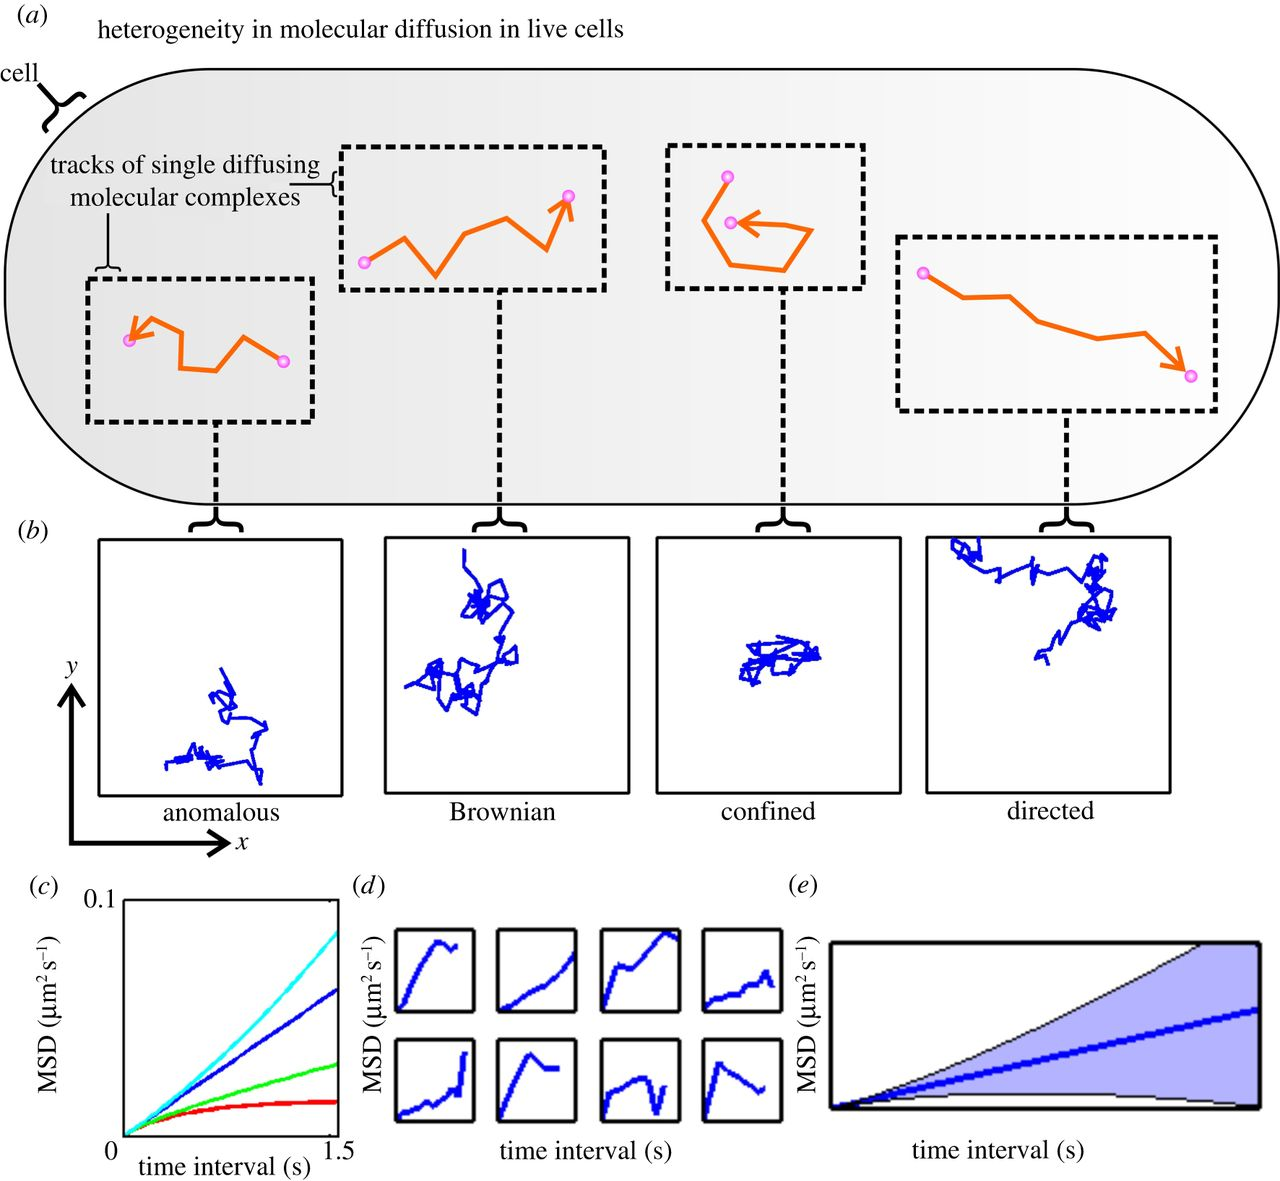
\includegraphics[width=75mm]{MSD.jpg}}
\caption{Overview of MSD to calculate track behavior \citep{Robson}. (a) Depicts simplified orange tracks of pink single-molecule incidences in a live cell. (b) Experimental tracking of incidences depicting the four main modes of diffusion. (c) Idealized forms of MSD as directed (cyan), normal/Brownian (blue), anomalous (green), and confined (red) diffusion. (d) Individual MSD plots. (e) Average MSD plot with blue shading indicating stochastic spread.}\label{fig:09}
\end{figure}

\subsubsection{Diffusion Coefficient}

While MSD is a useful measure of diffusion behavior, the diffusion coefficient (DCoef) is a measure of diffusion rate. By solving for the probability density function of a particle in n-dimensions (in this case, two) from Fick's second law for a n-dimensional differential equation for diffusion, one can actually derive the MSD from a known DCoef. However, since it is much easier to empirically calculate the MSD of a Brownian particle using the procedure described, the MSD experimentally is used to calculate the track's DCoef. In order to calculate this value, we rely on Einstein's theory on Brownian motion and the relationship between the MSD of a particle following a random walk and the time elapsed \citep{Einstein}:

\begin{equation}
\frac{\partial C(\vec{r}, \Delta t)}{\partial \Delta t} = D \nabla^2C(\vec{r}, \Delta t)\label{eq:07}
\end{equation}

where $C$ represents the particles per unit volume with a n-dimensional $\vec{r}$, $D$ is the DCoef, and $\Delta t$ is the time elapsed. Solving for $C$:

\begin{equation}
C(\vec{r}, \Delta t) = \frac{1}{(2 \pi D \Delta t)^{d/2}}\exp{\left( -\frac{r^2}{2 D \Delta t} \right)}\label{eq:08}
\end{equation}

multipliying the diffusion equation by $r^2$ and integrating over space:

\begin{equation}
\Big \langle \Delta r^2(\tau) \Big \rangle = 2 * d * D * \Delta t\label{eq:09}
\end{equation}

where $d$ is the dimensionality (in this case, two). Thus:

\begin{equation}
D = \frac{\Big \langle \Delta r^2(\tau) \Big \rangle}{4 \Delta t}  = \frac{MSD(\tau)}{4 \Delta t} \label{eq:10}
\end{equation}

While the MSD is useful in providing behavioral information about diffusion, the DCoef is a robust summary measurement that quantifies the diffusivity rate of the system as a whole. Plotting the logarithmically transformed individual DCoefs allows comparisons to expected distributions of DCoefs for a homogeneous population of diffusers.

\subsubsection{Dwell Times}

Dwell time is the simplest analytic tool that is used to measure the residence time of single-molecule tracks. This is essentially the track's lifetime in milliseconds and is calculated using the imaging exposure time and the frame duration. Because fluorescence resonance energy transfer (FRET) technology closely relies on distance-dependent interactions between two (donor and acceptor) fluorophores, measuring dwell times is a simple way to measure the temporal length of the transition dipole interaction. However, a limitation to this measurement is that photobleaching can often occur both in the presence and absence of acceptors through fluorophore decay and irreversible structural cleaving \citep{Liu}. This effect underestimates dwell times of tracks with prolonged or hyper-intense light exposure.


\subsubsection{Cumulative Distribution Function}

The CDF, or more precisely the cumulative radial distribution function, calculates the probability of the next position for a given time lag $\Delta t$ to be within a radius $r$ of its previous position. It can be considered as an alternative method to measuring the diffusivity. This cumulative radial distribution of displacements describes information about experimental diffusion heterogeneity, but relies on a large sample size of displacements \citep{Vrljic}.

The first step in this process involves constructing the displacement CDF for a particular time interval/lag by counting the fraction of displacements less than or equal to the displacement $r$. For assumed unconstrained Brownian diffusion of single-molecules, the fit CDF for the theoretical displacement CDF is modeled as:

\begin{equation}
P(r, \Delta t) = 1 - \exp{(-r^2/4D_{app} \Delta t)}\label{eq:11}
\end{equation}

where $D_{app}$ can therefore be calculated as the apparent DCoef each time lag $\Delta t$. While there are a minimal number of displacements required for an accurate fit, Monte Carlo random walk simulations can be used to determine that value. Empirically, it was found that if fewer than 10 displacements are used to fit the resulting displacement PDF, the value of the DCoef will be underestimated due to fitting artifacts from the CDF. Since having different track lengths can often skew the calculated apparent DCoef to longer trajectories, having at least 50 displacements per fit is optimal. Furthermore, ensuring that the track data has been trimmed at the same length before fitting provides an alternate method to ensure accurate apparent DCoef calculation.

\subsubsection{Hidden Markov Models}

Hidden Markov models (HMMs) represent a rather experimental technique in determining diffusion states. As target proteins and complexes in live cells often exhibit multiple diffusion constants, it would be an over-generalization to adopt the previously covered methods of calculating diffusion coefficients. As these single-molecule tracks rapidly switch between ``slow" and ``fast" diffusive states,  HMMs are particularly useful in differentiating diffusive states of both individual tracks and track sub-populations as a whole. HMMs compute the likelihood of a single-molecule track by taking into account both the distribution of displacements and the time-dependent switching of diffusivity. This method supports the statistical determinations of multiple diffusion coefficients as well as the kinetic and mechanistic rates of switching between these states (Figure \ref{fig:10}). 

As track data is composed of a sequence of trajectories, each track has a diffusivity state sequence $S = (s_1, s_2, s_3,..., s_n)$ of the single-molecule incidence at each step. For instance, state sequence (1, 1, 1, 2, 2, 2, 2) might imply that the molecule was in a certain diffusivity state 1 during the first three displacements but transitioned to state 2 for the next four displacements. By evaluating the probability of state switching, it is possible to learn about the kinetic reaction rates of certain cellular systems, as diffusivity transitions usually results from target molecules associating with or dissociating from other complexes of interest. Even though exact state sequences for tracks cannot be unambiguously determined, analyzing single-molecule data significantly benefits from the huge number of tracks and their time-steps to identify trends in state switching from a probabilistic sense.

The statistical model for displacement relies on track state numbers to be considered as a random sequence. Therefore, to calculate the probability observing a certain track, one has to sum all possible state sequences as such \citep{Yu}:

\begin{equation}
P_T(T|\Theta; K) = \sum_S \prod^n_{j=1} \frac{P(S) \exp{\big[ -\frac{1}{2} \Delta x_j^T {{\sum}_{s j}}^{-1} \Delta x_j \big]}}{2 \pi |{\sum}_{s j}|^{1/2}} \label{eq:12}
\end{equation}

where $P(S)$ is the probability of a particular sequence and $\Theta$ is the collection of all model parameters (eg. kinetic rates and state DCoefs) needed to calculate $P(S)$. Thus, the likelihood function is simply the product of all track sequence probabilities and the maximum likelihood estimation of the parameters can be done by attempting to maximize the likelihood function. Since possible $S$ sequences scales exponentially with track length, the summation task can be incredibly computationally exhaustive. This implementation of HMM explores the forward-backward HMM inference algorithm to avoid brute-force summation and assumes that track state sequences are time-independent Markov chains.

\begin{figure}[!tpb]
\centerline{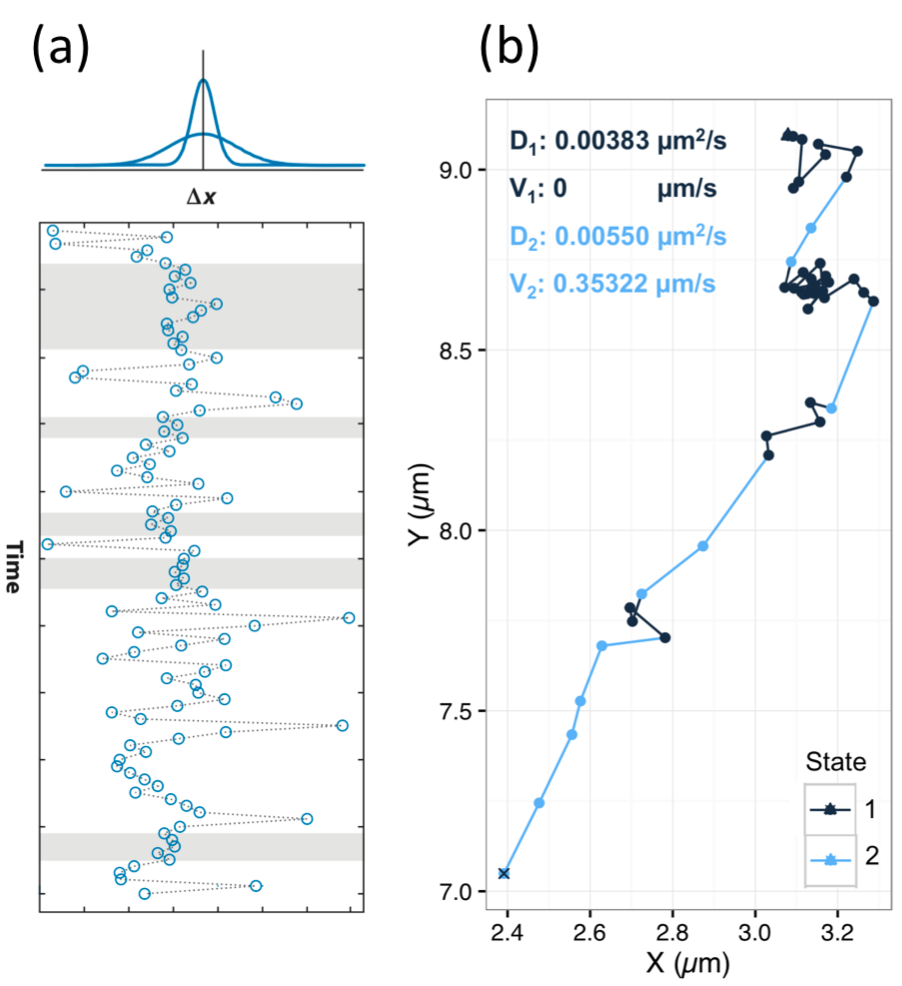
\includegraphics[width=65mm]{hmm.png}}
\caption{HMM justification and sample track states. (a, top) While a PDF of displacements might seem uniform and symmetric, it can only calculate an average apparent DCoef. (a, bottom) Plotting individual step displacements over time shows the vast variation in fast and slow-moving diffusive states. (b) Sample track with estimated DCoef states.}\label{fig:10}
\end{figure}

\begin{figure*}[!tpb]
\centerline{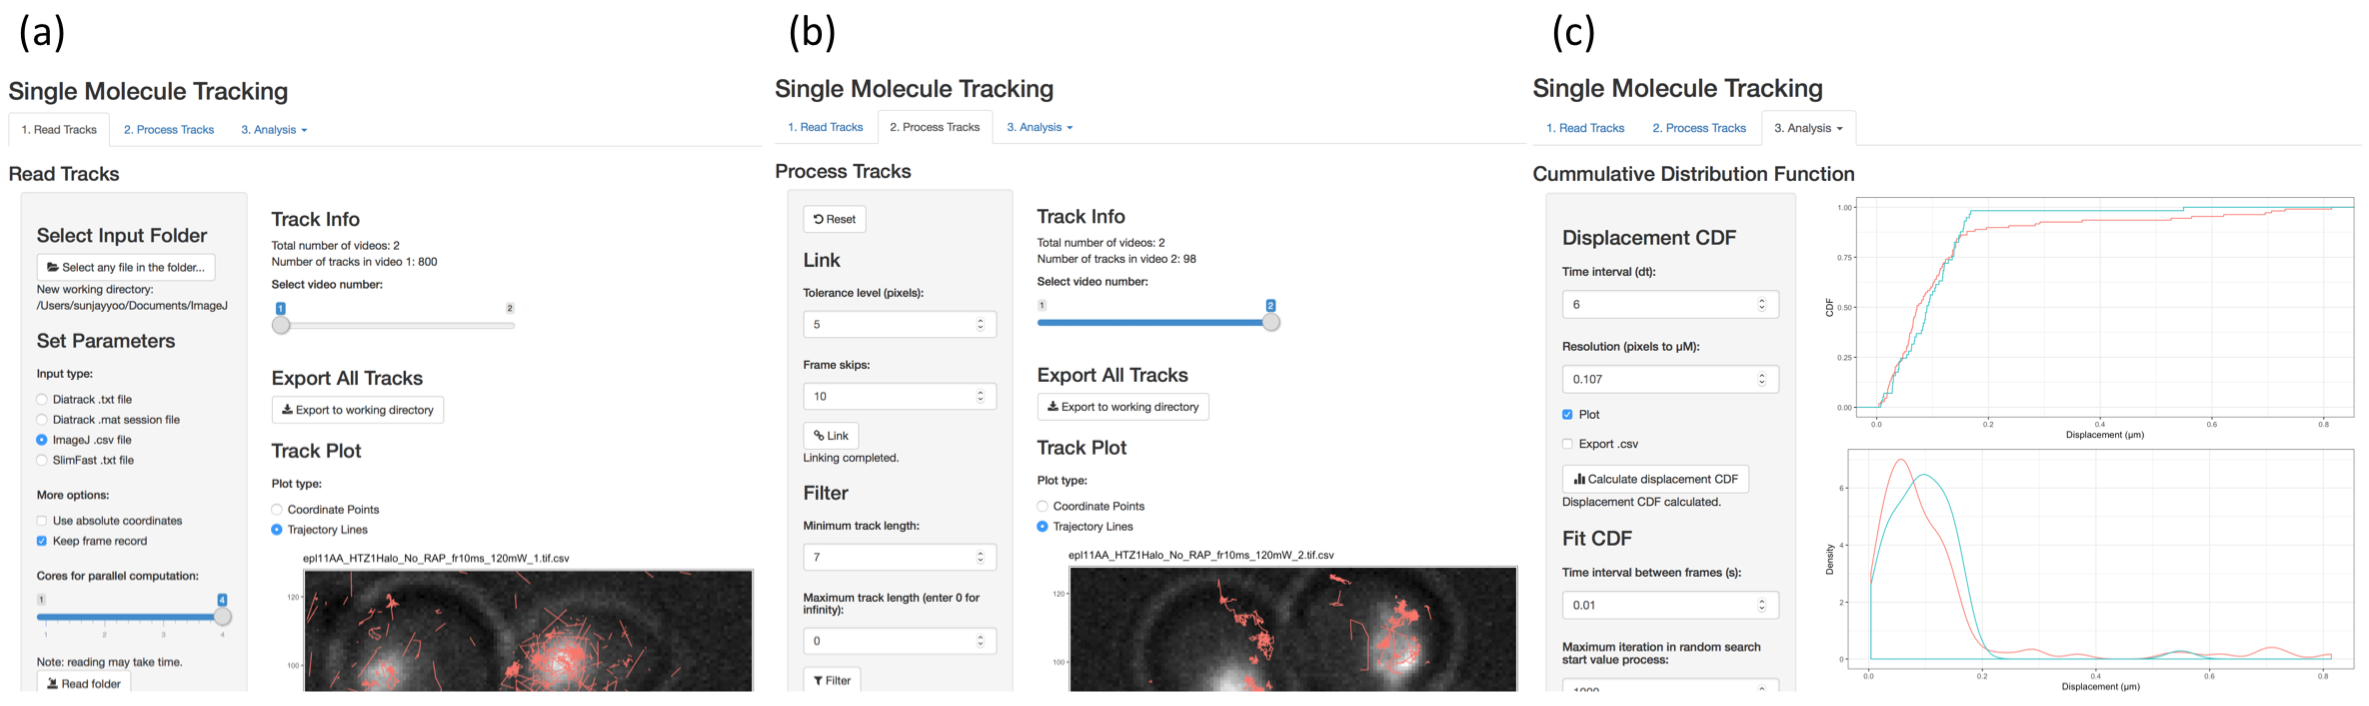
\includegraphics[width=175mm]{gui.png}}
\caption{Screenshots of the \textit{smt} user interface (note: only some features are depicted in these images). (a) Read tracks. (b) Process tracks. (c) Analysis. }\label{fig:11}
\end{figure*}

%\end{methods}
%%%%%%%%%%%%%%%%%%%%%%%%%%%%%%%%%%%%%%%%%%%%%%%%%%%%%%%%%%%%%%%%%%%%%%%%%%%%%%%%%%%%%%%%%%%%%%%%%%%%%%%%%%%%%%%%%%%%%%%%%%%%%%%%%%%%%%%%%%%%%%%%%%%%%%%%%%%%%%%%%%%%%%%%%%%%%%%%%%%%%%%%%%%%%%%%
\section{Results}

While \textit{smt} was intended to be used as a R software package, a full-featured graphical user interface using Shiny, JavaScript, HTML, and CSS was developed into the package to encourage use by those unfamiliar with the R language. 

The UI fully supports reading data produced from all localization software also supported by the base package. Furthermore, all processing features such as filtering, trimming, linking, merging, and masking have been implemented. In terms of analytic tools, all methods in the base software is also supported by the UI. Figure \ref{fig:11} provides screenshots of the three major components of the software pipeline.

Furthermore, the UI has the ability to export/re-import trackll data at any point, undo trackll modifications, and save plots and miscellaneous data from the suite of analytic tools. When reading and processing tracks, the UI displays the track plots that dynamically updates in the form of single-molecule incidences or trajectory lines over an image overlay. Altering miscellaneous system features such as the working directory and the number of cores for parallel computation is also integrated in to the UI. For educational and record-keeping purposes, the UI throws exceptions as necessary and tracks all commands in a history log in a format that can be entirely reproduced natively in a R script with code-comments for readability. This UI can be deployed purely on a remote R Studio Server or as a standalone website. The software is complete with full Roxygen documentation and help files for all primary functions.

\begin{figure}[!tpb]
\centerline{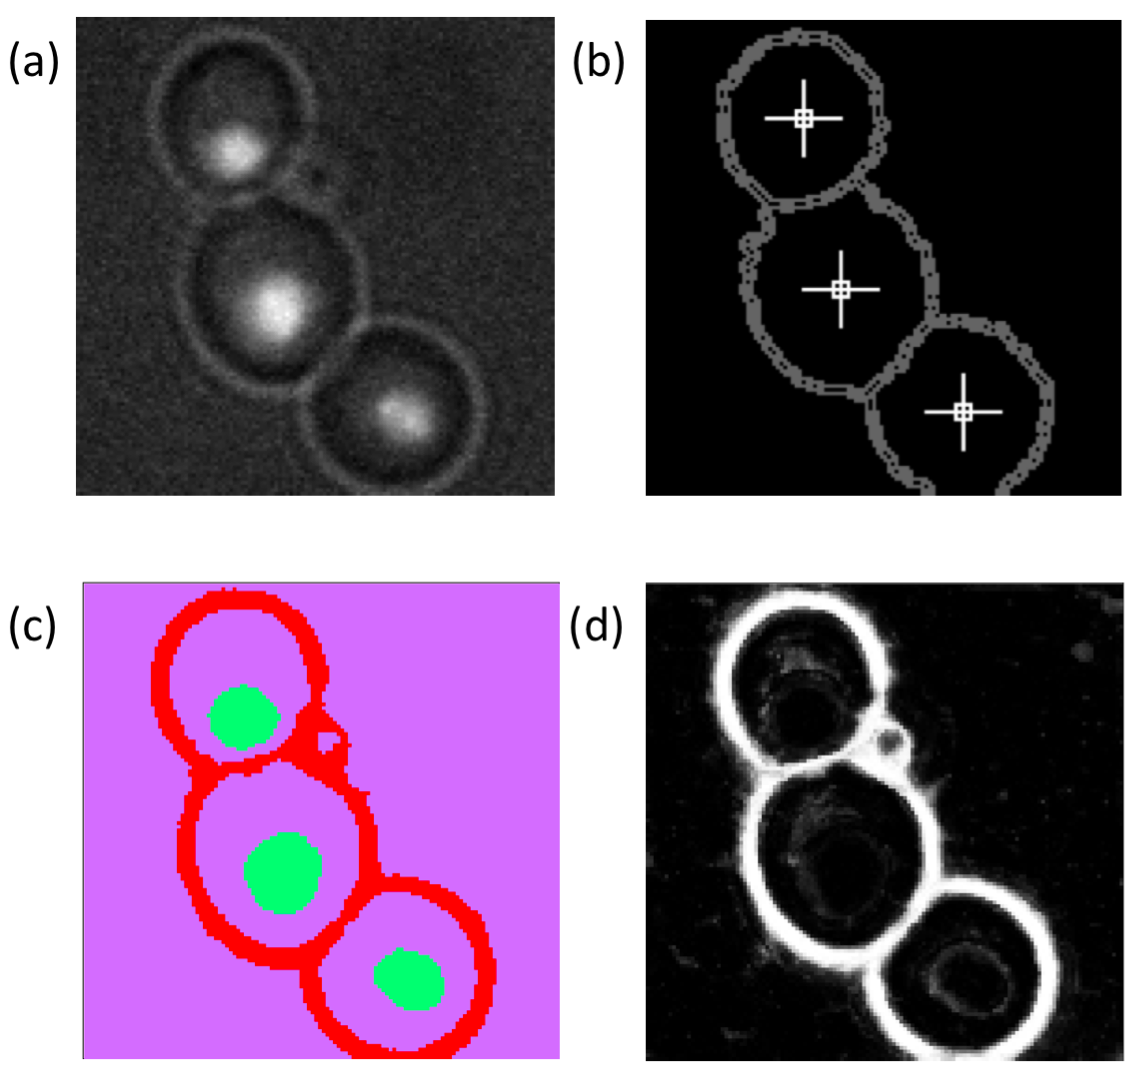
\includegraphics[width=65mm]{misc.png}}
\caption{Miscellaneous image analysis techniques using computer vision. (a) Sample raw image of a cell shot with a high-intensity flash. (b) Use of the Hough transform for circle detection and center estimation for mitosis and budding detection. (c) Morphological segmentation using machine learning techniques to detect cell and nuclei membranes. This could be an alternate method to manual threshold masking and could automate the image acquisition process by detecting optical sharpness using edge detection. (d) Alternate view with a segmented cell membrane.}\label{fig:12}
\end{figure}

%%%%%%%%%%%%%%%%%%%%%%%%%%%%%%%%%%%%%%%%%%%%%%%%%%%%%%%%%%%%%%%%%%%%%%%%%%%%%%%%%%%%%%%%%%%%%%%%%%%%%%%%%%%%%%%%%%%%%%%%%%%%%%%%%%%%%%%%%%%%%%%%%%%%%%%%%%%%%%%%%%%%%%%%%%%%%%%%%%%%%%%%%%%%%%%%
\section{Discussion}

While \textit{smt} already supports many of the common approaches to analyzing single-molecule data, these need to be refined as new analytic tools are also explored. While some operations (such as calculating square displacements) already have more efficient C/C++ replacements to be deployed, these function calls need to be further optimized and tested. Furthermore, tools such as HMM could be heavily refined by clarifying model parameters and vastly improving the performance. Existing statistical tools need more error analysis and stochastic processes need to be further studied. In terms of new features, it largely depends on the needs and experimental goals of the users. Nonetheless, many requests have already demonstrated novel potential. For example, through collecting intensity and goodness-of-fit data from the localization software, particle kymograph analysis could be attempted. Furthermore, as tracks are time-dependent data, transient cluster analysis along with time-specific diffusivity calculations could be implemented to gather more information on the effect of time on single-molecule kinetics. As it stands, there are already several computer vision tools that are already being explored, shown in Figure \ref{fig:12}. Nonetheless, \textit{smt} aims to be a software pipeline for single-molecule tracking that is constantly being developed and fine-tuned.
\\ \\
\raggedright{\textit{\footnotesize{(\textit{smt} is available on GitHub (https://github.com/snjy9182/smt) and coming to CRAN and Bioconductor repositories.)}}}


%%%%%%%%%%%%%%%%%%%%%%%%%%%%%%%%%%%%%%%%%%%%%%%%%%%%%%%%%%%%%%%%%%%%%%%%%%%%%%%%%%%%%%%%%%%%%%%%%%%%%%%%%%%%%%%%%%%%%%%%%%%%%%%%%%%%%%%%%%%%%%%%%%%%%%%%%%%%%%%%%%%%%%%%%%%%%%%%%%%%%%%%%%%%%%%%
\section*{Acknowledgements}

The author would like to thank Prof. Carl Wu, Dr. Sheng Liu, and all the members in Wu Lab (Johns Hopkins University) for providing amazing support and feedback on this project. The author also would like to thank Prof. Michael Schatz for facilitating this research process and providing valuable insight and inspiration on the computational biomedical field.

%%%%%%%%%%%%%%%%%%%%%%%%%%%%%%%%%%%%%%%%%%%%%%%%%%%%%%%%%%%%%%%%%%%%%%%%%%%%%%%%%%%%%%%%%%%%%%%%%%%%%%%%%%%%%%%%%%%%%%%%%%%%%%%%%%%%%%%%%%%%%%%%%%%%%%%%%%%%%%%%%%%%%%%%%%%%%%%%%%%%%%%%%%%%%%%%

%\bibliographystyle{natbib}
%\bibliographystyle{achemnat}
%\bibliographystyle{plainnat}
%\bibliographystyle{abbrv}
\bibliographystyle{bioinformatics}
%\bibliographystyle{plain}
%\bibliography{Document}


\begin{thebibliography}{}

\bibitem[Coleman \textit{et~al}., 2015]{Coleman}
Coleman,R.A. \textit{et~al}. (2015) Imaging Transcription: Past, Present, and Future. \textit{Cold Spring Harbor Symposia on Quantitative Biology}, \textbf{80}, 1--8.

\bibitem[Einstein, 1905]{Einstein}
Einstein,A. (1905) On the movement of small particles suspended in a stationary liquid demanded by the molecular-kinetic theory of heat. \textit{Annalen der Physik (Leipzig)}, \textbf{17}, 549--560.

\bibitem[Liu {\it et~al}., 2015]{Liu} Liu,Z., Lavis,L.D., Betzig,E. (2015) Imaging Live-Cell Dynamics and Structure at the Single-Molecule Level, {\it Molecular Cell}, {\bf 58}. 644--659

\bibitem[Manzo {\it et~al}., 2015]{Manzo} Manzo,C., Garcia-Parajo,M.F. (2015) A review of progress in single particle tracking: from methods to biophysical insights, {\it Reports on Progress in Physics}, {\bf 78}.

\bibitem[Monnier {\it et~al}., 2012]{Monnier} Monnier,N. \textit{et~al}. (2012) Bayesian approach to MSD-based analysis of particle motion in live cells., {\it Biophysics Journal}, {\bf 103}. 616--626

\bibitem[Plank {\it et~al}., 2009]{Plank} Plank,M. \textit{et~al}. (2009) Millisecond Timescale Slimfield Imaging and Automated Quantification of Single Fluorescent Protein Molecules for Use in Probing Complex Biological Processes, {\it Integrative Biology}, {\bf 1}. 601--612

\bibitem[Robson {\it et~al}., 2012]{Robson} Robson,A., Burrage,K., Leake,M.C. (2012) Inferring diffusion in single live cells at the single-molecule level, {\it Philosophical Transactions of The Royal Society}, {\bf 368}.

\bibitem[Venables \textit{et~al}. (2002)]{Venables}
Venables,W.N. \textit{et~al}. (2002) Density Estimation, \textit{Modern Applied Statistics with S}, 4th edn. Springer, 130--131.

\bibitem[Vrljic {\it et~al}., 2007]{Vrljic} Vrjlic,M., Nishimura,S.Y., Moerner,W.E. (2007) Single-Molecule Tracking, {\it Methods in Molecular Biology}, {\bf 398}. 193--219

\bibitem[Yu, 2016]{Yu}
Yu,J. (2016) Single-Molecule Studies in Live Cells. \textit{Annual Review of Physical Chemistry}, \textbf{67}, 565--585.

\end{thebibliography}
\end{document}